% Slides for 2025-02-03
% To create a slide, use the following:
% \begin{frame}{TITLE}
%     BODY
% \end{frame}

% To create a slide with a bullet list, use the following:
% \begin{frame}{TITLE}
%     \begin{itemize}
%         \item ITEM 1
%         \item ITEM 2
%     \end{itemize}    
% \end{frame}

% To create a slide with numbered list, use the following:
% \begin{frame}{TITLE}
%     \begin{enumerate}
%         \item ITEM 1
%         \item ITEM 2
%     \end{enumerate}
% \end{frame}

% To create a slide with a graphic:
% 1. Add the graphic to this folder (named picture.png)
% 2. Use the following:
% \begin{frame}{TITLE}
%     \centering
%     \includegraphics[height=0.7\textheight,width=0.7\textwidth,keepaspectratio]{picture.png}
% \end{frame}

% To create a slide with two columns, use the following:
% \begin{frame}{TITLE}
%     \begin{columns}
%         \begin{column}{0.5\textwidth}
%             COLUMN 1 BODY
%         \end{column}
%         \begin{column}{0.5\textwidth}
%             COLUMN 2 BODY
%         \end{column}
%     \end{columns}
% \end{frame}


\begin{frame}{What is Meshtastic?}
    \centering
    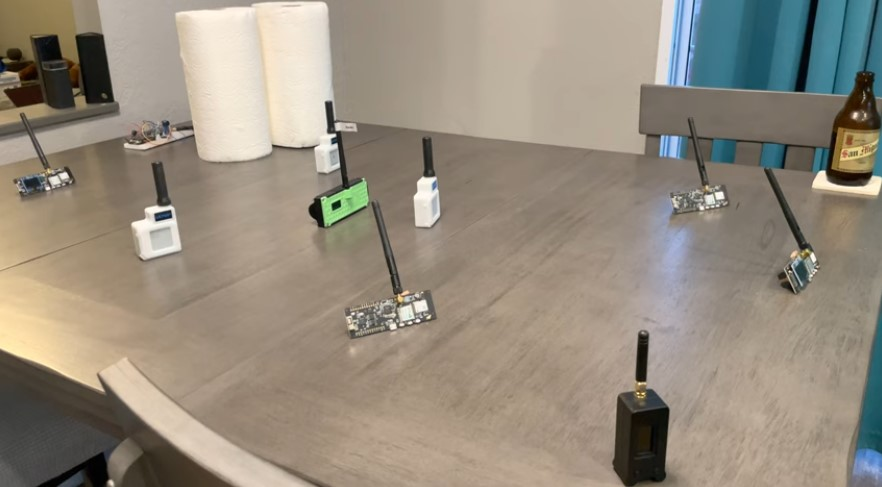
\includegraphics[height=0.7\textheight,width=0.7\textwidth,keepaspectratio]{images/rtt/mesh.jpg}\\
    Open source mesh network with LoRa
\end{frame}

\begin{frame}{Lower level features}
    \begin{enumerate}
        \item Managed flooding with minimal redundant rebroadcasts
        \item Messaging using implicit or explicit ACKs
        \item CSMA/CA with adaptive backoff
        \item Regular basic info broadcasts (IDs, GPS, etc)
    \end{enumerate}
\end{frame}

\begin{frame}{RTT Tower Comms Package}
    \centering
    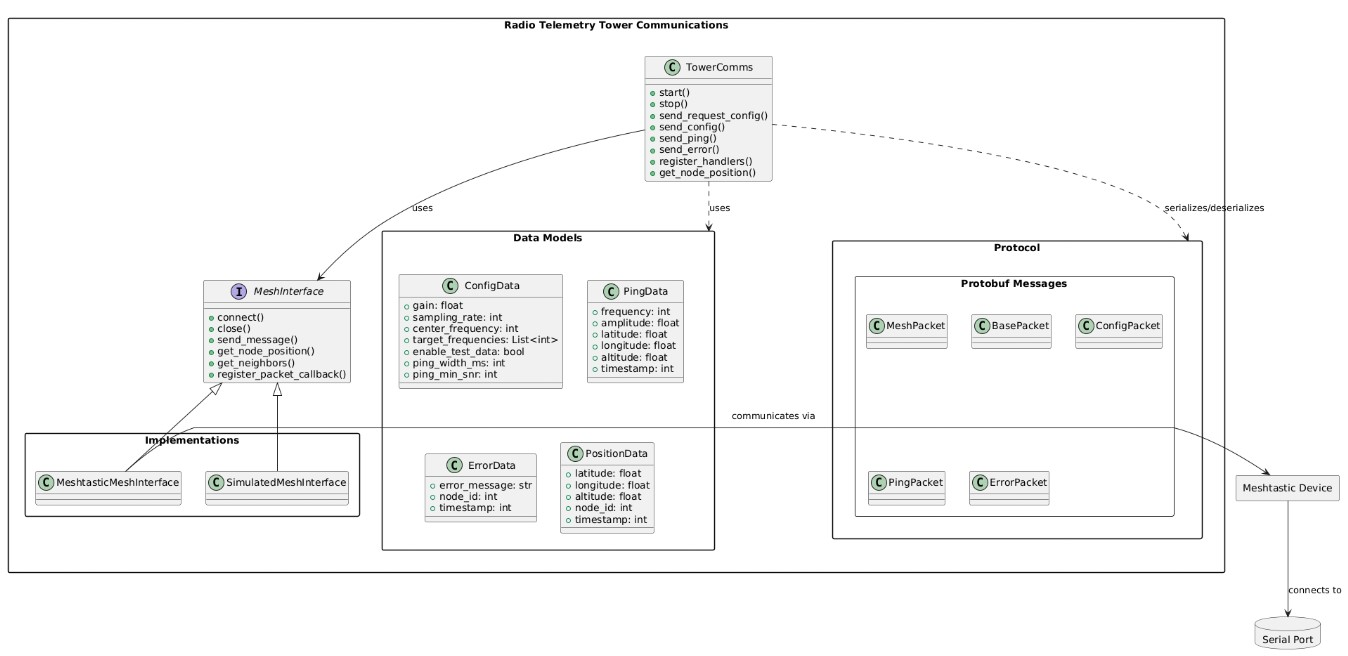
\includegraphics[height=0.7\textheight,width=0.7\textwidth,keepaspectratio]{images/rtt/tower_comms.jpg}
\end{frame}

\begin{frame}{Misc. Updates}
    \begin{enumerate}
        \item GCS simulator now works on Mac
        \item Working on save/laod flight data
        \item Strealined FDS configuration
    \end{enumerate}
\end{frame}